\documentclass{article}
\usepackage{graphicx}
\usepackage{subcaption}
\pagestyle{empty}
\begin{document}
\begin{figure}[ht] 
\centering Velocity plots
  \begin{subfigure}[b]{0.5\linewidth}      
    \centering    
    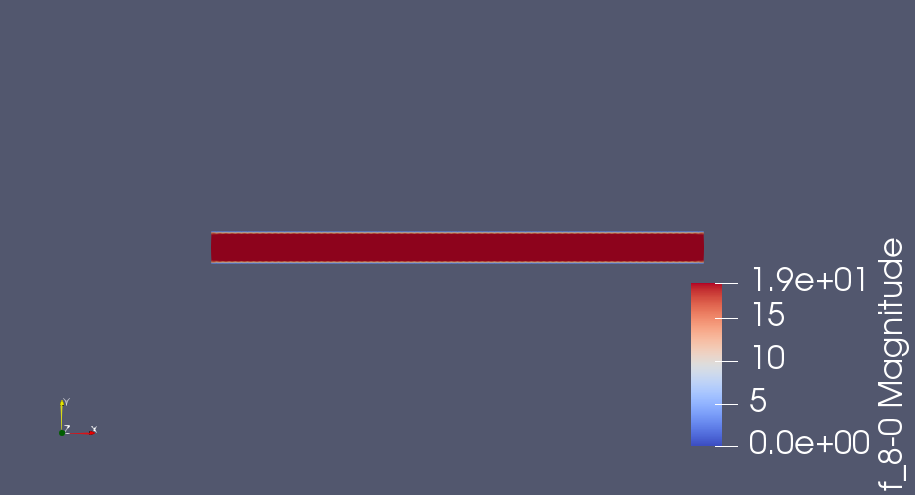
\includegraphics[width=1\linewidth]{velocity_time_0.png} 
    \caption{$t=0.0$ (sixth cycle)} 
    \label{fig7:a} 
    \vspace{4ex}
  \end{subfigure}%% 
  \begin{subfigure}[b]{0.5\linewidth}
    \centering
    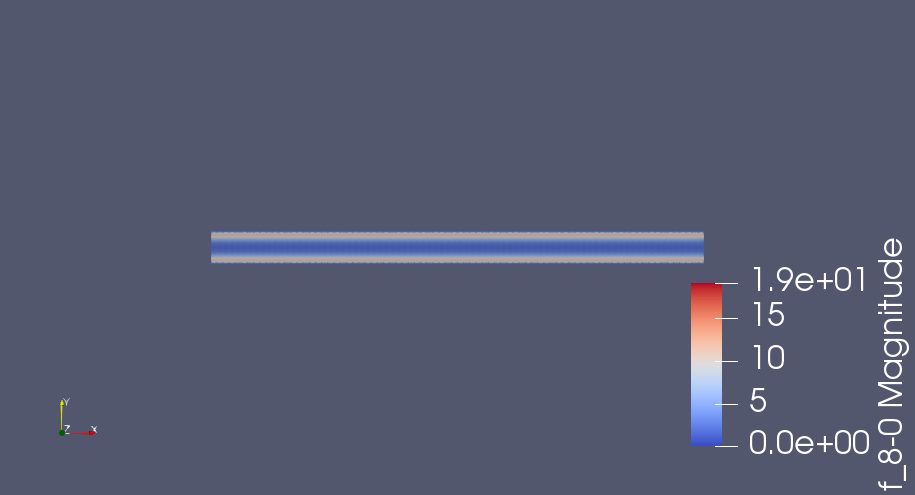
\includegraphics[width=1\linewidth]{velocity_time_025.png} 
    \caption{$t=0.25$ (sixth cycle)} 
    \label{fig7:b} 
    \vspace{4ex}
    \end{subfigure} 
  \begin{subfigure}[b]{0.5\linewidth}
    \centering
    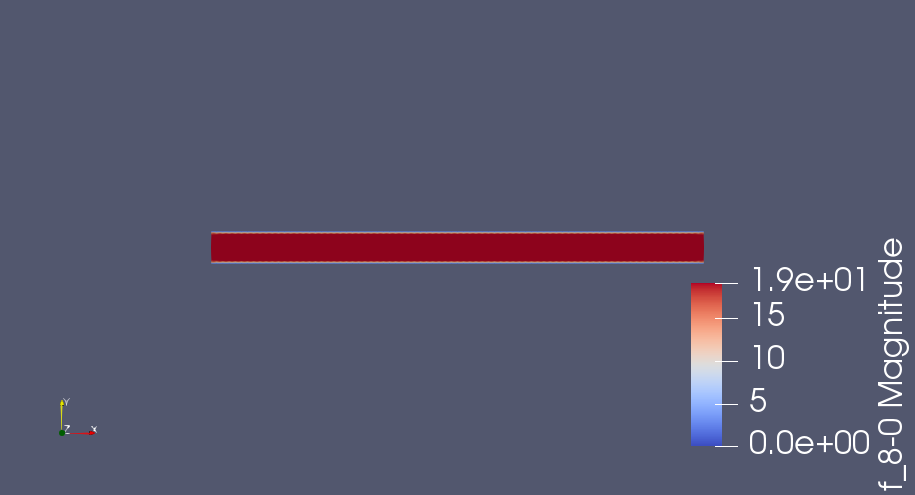
\includegraphics[width=1\linewidth]{velocity_time_050.png} 
    \caption{$t=0.50$ (sixth cycle)} 
    \label{fig7:c} 
  \end{subfigure}%%
  \begin{subfigure}[b]{0.5\linewidth}
    \centering
    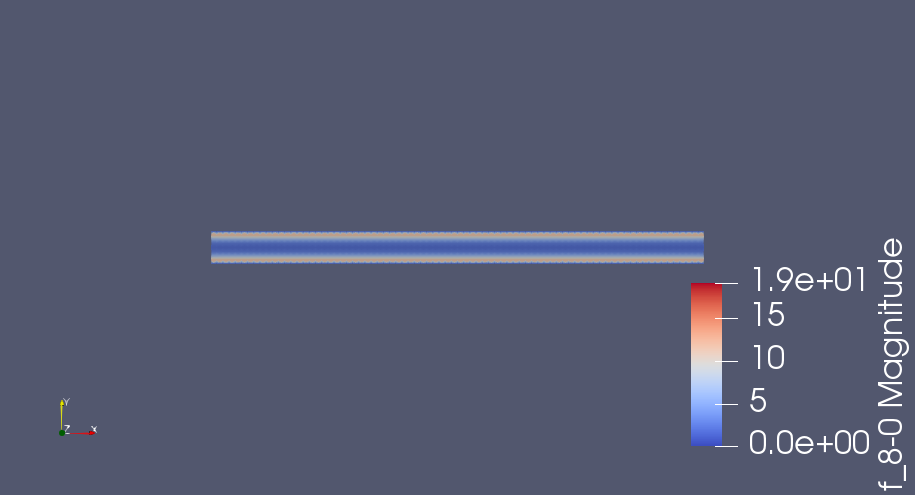
\includegraphics[width=1\linewidth]{velocity_time_075.png} 
    \caption{$t=0.75$ (sixth cycle)} 
    \label{fig7:d} 
  \end{subfigure} 
  \caption{Illustration of various images}
  \label{fig7} 
\end{figure}

\begin{figure}[ht] 
\centering Pressure plots
  \begin{subfigure}[b]{0.5\linewidth}      
    \centering    
    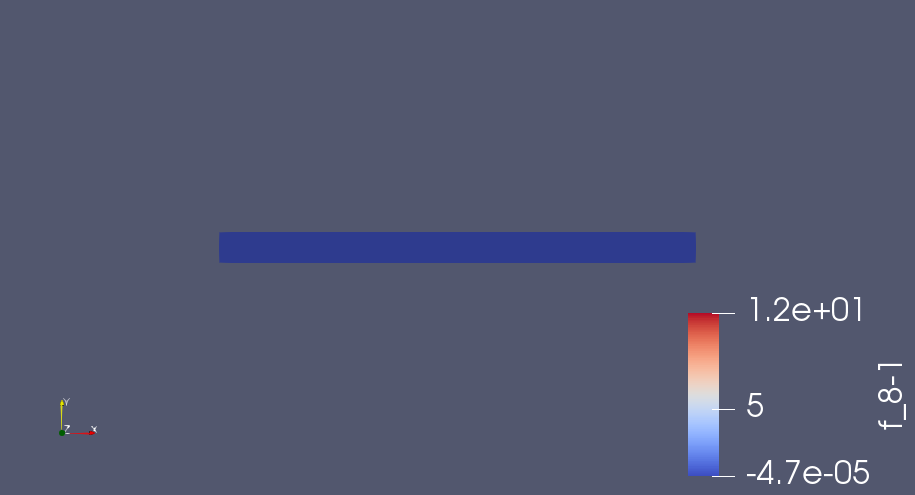
\includegraphics[width=1\linewidth]{pressure_time_0.png} 
    \caption{$t=0.0$ (sixth cycle)} 
    \label{fig7:a} 
    \vspace{4ex}
  \end{subfigure}%% 
  \begin{subfigure}[b]{0.5\linewidth}
    \centering
    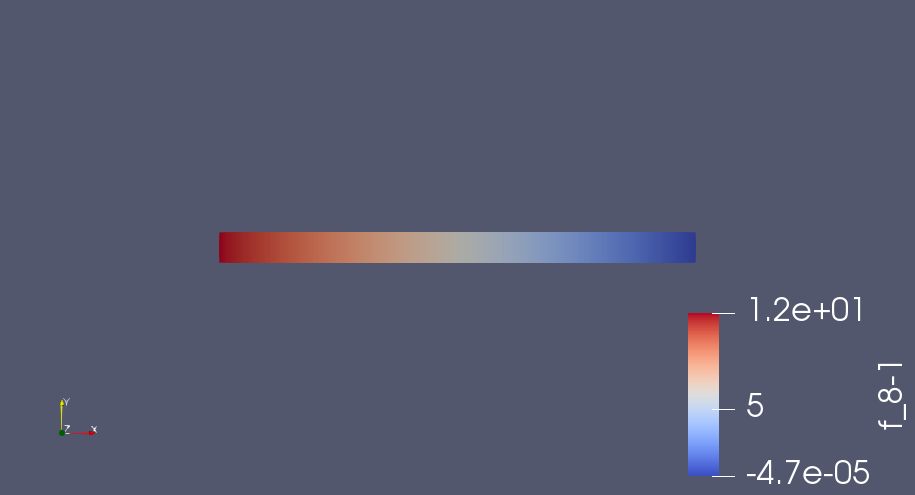
\includegraphics[width=1\linewidth]{pressure_time_025.png} 
    \caption{$t=0.25$ (sixth cycle)} 
    \label{fig7:b} 
    \vspace{4ex}
    \end{subfigure} 
  \begin{subfigure}[b]{0.5\linewidth}
    \centering
    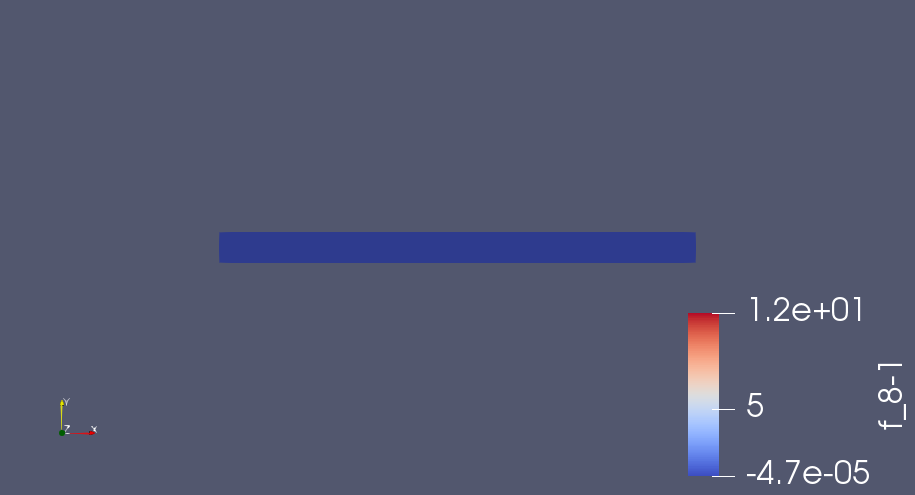
\includegraphics[width=1\linewidth]{pressure_time_050.png} 
    \caption{$t=0.50$ (sixth cycle)} 
    \label{fig7:c} 
  \end{subfigure}%%
  \begin{subfigure}[b]{0.5\linewidth}
    \centering
    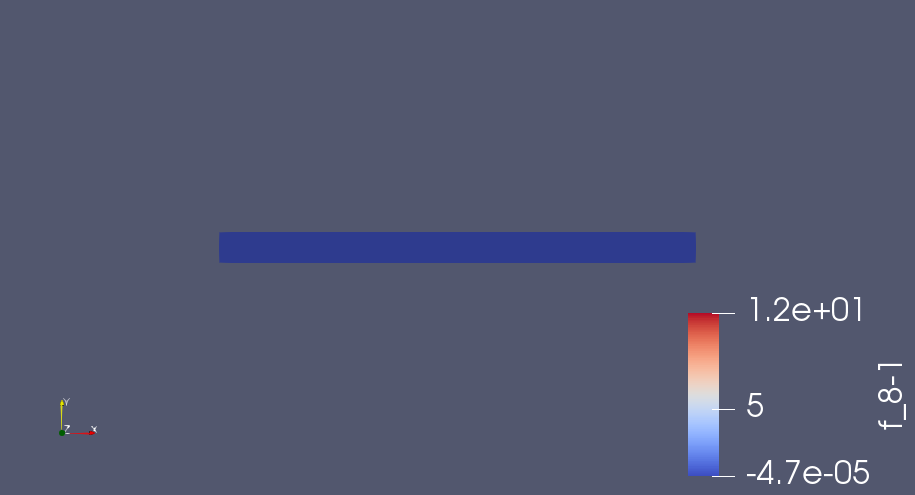
\includegraphics[width=1\linewidth]{pressure_time_075.png} 
    \caption{$t=0.75$ (sixth cycle)} 
    \label{fig7:d} 
  \end{subfigure} 
  \caption{Illustration of various images}
  \label{fig7} 
\end{figure}


\end{document}
